% Options for packages loaded elsewhere
\PassOptionsToPackage{unicode}{hyperref}
\PassOptionsToPackage{hyphens}{url}
%
\documentclass[
]{book}
\usepackage{lmodern}
\usepackage{amssymb,amsmath}
\usepackage{ifxetex,ifluatex}
\ifnum 0\ifxetex 1\fi\ifluatex 1\fi=0 % if pdftex
  \usepackage[T1]{fontenc}
  \usepackage[utf8]{inputenc}
  \usepackage{textcomp} % provide euro and other symbols
\else % if luatex or xetex
  \usepackage{unicode-math}
  \defaultfontfeatures{Scale=MatchLowercase}
  \defaultfontfeatures[\rmfamily]{Ligatures=TeX,Scale=1}
\fi
% Use upquote if available, for straight quotes in verbatim environments
\IfFileExists{upquote.sty}{\usepackage{upquote}}{}
\IfFileExists{microtype.sty}{% use microtype if available
  \usepackage[]{microtype}
  \UseMicrotypeSet[protrusion]{basicmath} % disable protrusion for tt fonts
}{}
\makeatletter
\@ifundefined{KOMAClassName}{% if non-KOMA class
  \IfFileExists{parskip.sty}{%
    \usepackage{parskip}
  }{% else
    \setlength{\parindent}{0pt}
    \setlength{\parskip}{6pt plus 2pt minus 1pt}}
}{% if KOMA class
  \KOMAoptions{parskip=half}}
\makeatother
\usepackage{xcolor}
\IfFileExists{xurl.sty}{\usepackage{xurl}}{} % add URL line breaks if available
\IfFileExists{bookmark.sty}{\usepackage{bookmark}}{\usepackage{hyperref}}
\hypersetup{
  pdftitle={LA SOLUCIÓN DEFINITIVA PARA OBTENER UTILIDADES COMO LOS GRANDES INVERSIONISTAS},
  pdfauthor={Granja de Inversiones},
  hidelinks,
  pdfcreator={LaTeX via pandoc}}
\urlstyle{same} % disable monospaced font for URLs
\usepackage{longtable,booktabs}
% Correct order of tables after \paragraph or \subparagraph
\usepackage{etoolbox}
\makeatletter
\patchcmd\longtable{\par}{\if@noskipsec\mbox{}\fi\par}{}{}
\makeatother
% Allow footnotes in longtable head/foot
\IfFileExists{footnotehyper.sty}{\usepackage{footnotehyper}}{\usepackage{footnote}}
\makesavenoteenv{longtable}
\usepackage{graphicx}
\makeatletter
\def\maxwidth{\ifdim\Gin@nat@width>\linewidth\linewidth\else\Gin@nat@width\fi}
\def\maxheight{\ifdim\Gin@nat@height>\textheight\textheight\else\Gin@nat@height\fi}
\makeatother
% Scale images if necessary, so that they will not overflow the page
% margins by default, and it is still possible to overwrite the defaults
% using explicit options in \includegraphics[width, height, ...]{}
\setkeys{Gin}{width=\maxwidth,height=\maxheight,keepaspectratio}
% Set default figure placement to htbp
\makeatletter
\def\fps@figure{htbp}
\makeatother
\setlength{\emergencystretch}{3em} % prevent overfull lines
\providecommand{\tightlist}{%
  \setlength{\itemsep}{0pt}\setlength{\parskip}{0pt}}
\setcounter{secnumdepth}{5}
\usepackage{booktabs}
\usepackage{float}
\usepackage[left=3cm,right=3cm,top=6cm,bottom=6cm]{geometry}
\ifxetex
  \usepackage{polyglossia}
  \setmainlanguage{spanish}
  % Tabla en lugar de cuadro
  \gappto\captionsspanish{\renewcommand{\tablename}{Tabla}  
          \renewcommand{\listtablename}{Índice de tablas}}
\else
  \usepackage[spanish,es-tabla]{babel}
\fi
\newlength{\cslhangindent}
\setlength{\cslhangindent}{1.5em}
\newenvironment{cslreferences}%
  {\setlength{\parindent}{0pt}%
  \everypar{\setlength{\hangindent}{\cslhangindent}}\ignorespaces}%
  {\par}

\title{LA SOLUCIÓN DEFINITIVA PARA OBTENER UTILIDADES COMO LOS GRANDES INVERSIONISTAS}
\author{Granja de Inversiones}
\date{2021-10-21}

\begin{document}
\maketitle

{
\setcounter{tocdepth}{1}
\tableofcontents
}
\hypertarget{portada}{%
\chapter*{Portada}\label{portada}}
\addcontentsline{toc}{chapter}{Portada}

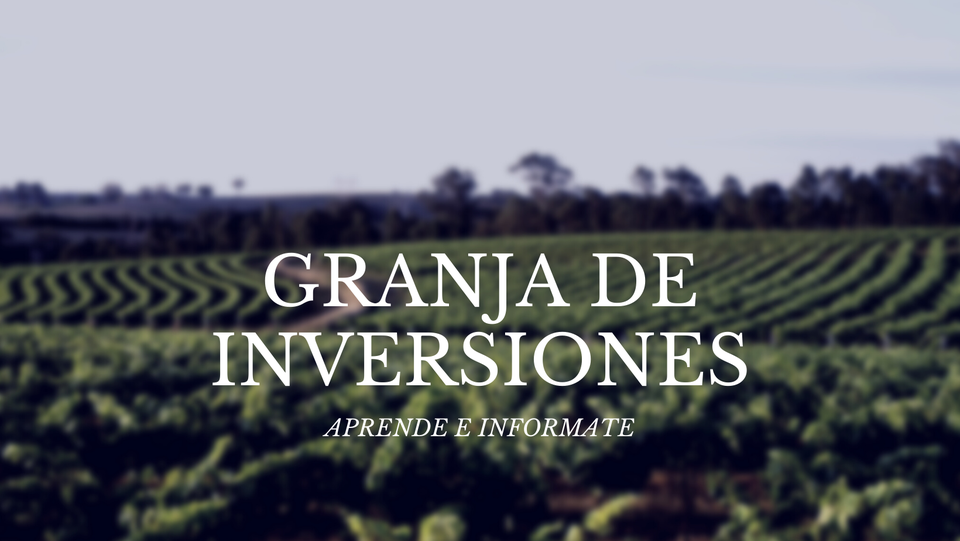
\includegraphics[width=1\linewidth,height=1\textheight]{imagenes/Granja}

\hypertarget{los-males-que-nos-afectan-a-todos}{%
\chapter{LOS MALES QUE NOS AFECTAN A TODOS}\label{los-males-que-nos-afectan-a-todos}}

La crisis a nivel global generada por el COVID-19, que afectó a Colombia de manera particular, ha puesto al descubierto otras problemáticas que el país viene arrastrando desde varios años atrás, y que complejizan aún más la severidad de los estragos actuales y futuros. Por una parte, el nivel de desaprobación histórica que carga el actual gobierno, producto de decisiones polémicas, incumplimientos de promesas, niveles de inseguridad, corrupción por las nubes y desconfianza generalizada en sus instituciones, ha exacerbado el nivel de incertidumbre del país, a dimensiones preocupantes en el contexto regional y mundial.

Otros factores que afectan de manera directa el entorno económico interno, corresponden al incremento sustancial en la tasa de desempleo, que se ubicó en 15,9\% en 2020, lo que significa un aumento de 5,4 puntos porcentuales más, frente al 10,5 \% de 2019 (Economı́a (\protect\hyperlink{ref-Portafolio2021Desempleo}{2021})). Adicionalmente las debilidades sustanciales en cuanto a cobertura social y el incremento de la pobreza ``\ldots{} El DANE reveló que la pobreza en el país se incrementó de 35,7\% en 2019, a 42,5\% en 2020. Casi un 7\%. Esto quiere decir que pasamos de 17,5 millones de personas pobres (que no era poco) a 21,02 millones\ldots{}'' (Rojas Mantilla. (\protect\hyperlink{ref-Rojas2021Concejo}{2021})).

Pero estas cifras críticas no son culpa exclusiva de la pandemia, la progresiva destrucción de la economía colombiana empezó con la apertura económica proclamada por el entonces Presidente Cesar Gaviria, que mediante un Compes en 1990, abrió las puertas del país a una exposición gradual al mercado global, ``\ldots{} Con el ánimo no solo de mejorar sus relaciones comerciales, sino de incentivar él crecimiento de la industria nacional gracias a la competencia con los demás países y una mejor disponibilidad tanto de bienes como de consumidores\ldots{}'' (Semana (\protect\hyperlink{ref-Semana2018Apertura}{2018})).

Para ese momento la agricultura y la manufactura eran los principales renglones productivos del país, y representaban el 22.3\% y el 21.1\% del Producto Interno Bruto - PIB, mientras que la banca o sector financiero solo llegaba al 15\%. Para 2018 las cifras dieron un vuelco total, al punto que la banca pasó a convertirse en el principal renglón de la economía al aportar el 21.2\% del PIB, mientras que la agricultura y la manufactura pasaron a desempeñar papeles secundarios al aportar el 6.3\% y el 10.9\% respectivamente (Semana (\protect\hyperlink{ref-Semana2018Apertura}{2018})).

La política neoliberal que desde ese entonces gobierna el país, lanzó a nuestra economía de manera prematura a un río caudaloso (mercado mundial) sin flotador, destacándose la ausencia de una estrategia de producción nacional que incentivara la generación de valor agregado. Al contrario, se enfocó casi que exclusivamente a la lucha armada, que paulatinamente fue perdiendo contra diversas estructuras ilegales, alimentadas por el narcotráfico y que terminaron permeando las más altas esferas del poder público.

Como resultado, se tiene un país de vocación rural con una industria agrícola destruida, que se posiciona como el mayor importador de productos alimenticios y agropecuarios de América Latina (Agricultores Colombianos (\protect\hyperlink{ref-SAC2019Agricultores}{2019})), en donde el 42.5\% de la población total se encuentra en situación de pobreza (Salazar Sierrra (\protect\hyperlink{ref-Republica2021millones}{2021})).


\includegraphics[width=1\linewidth,height=0.3\textheight]{imagenes/Granja1}

\hypertarget{ganadores-y-perdedores}{%
\chapter{GANADORES Y PERDEDORES}\label{ganadores-y-perdedores}}

El sistema financiero, responsable de jalonar la economía nacional (según el aporte al PIB) y que en la opinión de la mayoría de expertos, permite disminuir la pobreza al canalizar el ahorro familiar hacia la inversión, además de reducir el costo del capital y de transacción, facilitar la distribución temporal del gasto, estimular el crecimiento económico, distribuir y diversificar el riesgo. No cumple dichas afirmaciones, ya que el verdadero objetivo y la tendencia general en una economía de mercado es acumular capital, y sus decisiones económicas están determinadas por las expectativas de ganancias, que le permitan a los dueños y accionistas concentrar sus utilidades, mientras la mayoría de la población asume las pérdidas de las operaciones financieras (Guerrero, 2017).

Mientras que para 2010 las utilidades netas del sistema financiero colombiano rondaban los \$8.7 Billones (Portafolio, 2010), entre enero y septiembre de 2020 triplicaban esa cifra, con un total de ganancias que ascendían a los \$24.25 Billones, valor mucho menor al mismo periodo de 2019, donde se llegó a los \$74.78 Billones (Vargas Rubio, 2020).

Pero este crecimiento no quiere decir que el sistema financiero se ha expandido, posicionando más actores en el mercado, u ofreciendo más alternativas de ahorro y de inversión que favorezca la competitividad y los beneficios al cliente; por el contrario en este ambiente de crisis permanente el estado cambió su papel de actor directo por el de regulador, se dieron fusiones, recompras, alianzas entre bancos y se fortaleció la concentración del patrimonio y activos bancarios en pocos grupos. Según datos de la Superintendencia Financiera, en el año 1985, existían 87 entidades de crédito, en 1996, 147, en 2004 57; para 2010 solo existían 23 (Guerrero, 2017) y en la actualidad todo el mercado está en poder de 13 grupos, que antes de competir, se articulan para salvaguardar las condiciones ventajosas de sus dueños y accionistas.

Para perpetuar dichas condiciones, el sistema ha estrechado los vínculos con el gobierno, que le permite el control del mercado, financiando las campañas políticas con mayor posibilidad de ganar, para después cobrar dividendos con leyes que cambian la regulación, por ejemplo la Ley 795 de 2003, que modificó las normas aplicadas al capital, establecidas en Ley 510 de 1999 (Guerrero, 2017)

Por otra parte, la población, víctima acostumbrada de la concentración de poderes y la desigualdad, ha visto como el desempleo en Colombia en el período 2001-2018, registró la tasa promedio (11.1\%) más alta entre las principales cinco economías de América Latina (Argentina, Brasil, Chile, Colombia y México), incluso superando el promedio de América Latina por más de 3.6 puntos porcentuales (Ramos \& Álvarez García, 2020). Para 2020, las cifras aumentaron significativamente en el mundo y en la región, no obstante, Colombia sigue como líder con una tasa promedio de 15.9\% para 2020, mientras que países como Brasil y Chile presentaron cifras de 13.5\% y 10.2\% respectivamente (Revista Semana, 2021).


\includegraphics[width=1\linewidth,height=0.3\textheight]{imagenes/Granja1}

\hypertarget{la-tecnologuxeda-social-una-nueva-esperanza}{%
\chapter{LA TECNOLOGÍA SOCIAL, UNA NUEVA ESPERANZA}\label{la-tecnologuxeda-social-una-nueva-esperanza}}

NA NUEVA ESPERANZA

Tradicionalmente la adquisición de acciones, la compra y venta de divisas, y el acceso a portafolios de inversión, estaban restringidos a personas y empresas con grandes capitales, que utilizaban estos medios para concentrar y acrecentar mucho más su riqueza.

Una persona que quisiera ahorrar alguna fracción de sus ingresos, para lograr objetivos como la compra de una vivienda, un vehículo, pagar estudios superiores, o simplemente hacer realidad ese viaje soñado, se tenía que resignar con abrir una cuenta de ahorros, un título de ahorro, abrir un Certificado de Depósito a Término -- CDT, o delegar el manejo de su capital en un Fondo de Cesantías.

Pero todas estas opciones tienen un denominador común; una utilidad excesivamente baja que deja las verdaderas ganancias en el sistema financiero y que empuja a la gente a abandonar sus aspiraciones y dedicarse al consumo inmediato, o depositar sus esperanzas en alternativas de origen informal y de muy alto riesgo, como las pirámides, con la expectativa de obtener un rendimiento mayor de su dinero.

El desarrollo tecnológico y el crecimiento de la conectividad y la capacidad de innovación, han permitido un nivel de comunicación e interacción social sin precedentes, el acceso al conocimiento, y la adquisición de innumerables productos y servicios. Adicionalmente, desde hace aproximadamente una década ha permitido el acceso a nuevos servicios bancarios y de pagos, así como la creación de nuevos ecosistemas colaborativos que abren un nuevo horizonte de servicios financieros innovadores y mucho más participativos (Rodríguez Fernández, 2017).

A este nuevo sector se le llama Fintech, y se caracteriza por la prestación de servicios financieros soportados a través de plataformas tecnológicas (finance - technology) y la presencia de una gran diversidad de operadores que favorecen la competencia y permiten disminuir considerablemente el margen de intermediación, en beneficio del cliente. Estas empresas son parte de la transformación digital, y permiten ofrecer un nuevo abanico de opciones y servicios financieros mediante la adopción de las nuevas herramientas digitales, el uso de la inteligencia artificial, la gestión de datos, o el desarrollo de criptomonedas (Rodríguez Fernández, 2017).


\includegraphics[width=1\linewidth,height=0.3\textheight]{imagenes/Granja1}

\hypertarget{financiaciuxf3n-colaborativa-inversiuxf3n-de-alto-impacto-y-utilidades-verdaderas}{%
\chapter{FINANCIACIÓN COLABORATIVA -- INVERSIÓN DE ALTO IMPACTO Y UTILIDADES VERDADERAS}\label{financiaciuxf3n-colaborativa-inversiuxf3n-de-alto-impacto-y-utilidades-verdaderas}}

Entre la gran diversidad de alternativas en el mercado Fintech, destaca el Crowdfunding o financiación colaborativa por su gran potencial de impacto a nivel social. Consiste en la aportación de pequeñas cantidades de dinero por parte de un gran número de individuos (economía participativa) a un proyecto determinado mediante el uso de plataformas tecnológicas interactivas (Rodríguez Fernández, 2017). Los proyectos pueden ser de diferente naturaleza con un riesgo igualmente variado, que define el nivel de utilidad ofrecida, en todo caso los beneficios prometidos son superiores a los modelos de inversión de la banca actual.

También hay diferentes modelos de financiación, el crowdfunding no financiero, que fue el modelo inicial y engloba dos tipos de plataformas: la primera, especializada en el recaudo de donaciones (donation - based crowdfunding), para apoyar proyectos sin ánimo de lucro de carácter social o cultural, y que permite hacer un seguimiento del nivel de financiación y de desarrollo del proyecto, así como la puesta en contacto de los financiadores, los promotores e incluso los beneficiarios. La segunda, que busca financiar proyectos generalmente innovadores, en los que el rendimiento tiene forma de recompensa (rewardbased); por ejemplo, el ofrecimiento de entradas para el estreno de una película financiada mediante esta opción.

Y el crowdfunding financiero, donde el financiador se convierte en inversionista al obtener una retribución en forma de interés o de dividendos fruto de su aporte. Así mismo, dentro de este grupo, se distinguen dos modelos, el de préstamos y bonos (lendingy debt-based) que ofrece una rentabilidad fija a un plazo establecido previamente, y el que ofrece una participación en el capital (equity), en donde el inversionista se convierte en socio del proyecto que está financiando y la utilidad depende del éxito del proyecto; en ambos casos quien emite el título de deuda o de inversión es la empresa que busca financiación (Rodríguez Fernández, 2017).


\includegraphics[width=1\linewidth,height=0.3\textheight]{imagenes/Granja1}

\hypertarget{como-se-puede-participar-en-financiaciuxf3n-colaborativa-en-colombia}{%
\chapter{COMO SE PUEDE PARTICIPAR EN FINANCIACIÓN COLABORATIVA, EN COLOMBIA}\label{como-se-puede-participar-en-financiaciuxf3n-colaborativa-en-colombia}}

Aunque el modelo crowdfunding en la modalidad de donación ya tenía algunos actores en Colombia, fue mediante la expedición del Decreto 1357 de 2018, que se regula el ambiente normativo de la financiación colaborativa en el país y que crea las condiciones para la iniciación del mercado en el país. El espíritu de esta Ley busca que se creen muchas plataformas de financiación que eviten los monopolios y fomenten la competencia, mediante las cuales cualquier persona pueda invertir en proyectos medianos y pequeños, con el ánimo de dinamizar la economía y obtener un retorno muy similar a las utilidades de los grandes fondos de inversión.

En el año 2020, se expidió el Decreto 1235, que tiene como principal fin, introducir cambios que motiven el movimiento del mercado, como el registro de las operaciones de los títulos valores, la posibilidad que la plataforma preste servicios de cobranza y que pueda ofrecer más de un objeto, es decir, los servicios de crowdfunding financiero y por donación, lo cual permite visibilidad de ciertos modelos de negocio, por ejemplo, compañías de beneficio e interés colectivo (BIC) que han venido adquiriendo un lugar en las preferencias de los empresarios.

No obstante, el cambio más relevante, y que se toma con gran expectativa en el mercado, es que el Decreto 1235 autoriza aumentar los montos de inversión, lo cual, abre nuevas alternativas frente a la envergadura de los posibles tipos de negocio que se creen, y representa una ventaja que permite a mercados con inversiones iniciales de altos montos, como, por ejemplo, el inmobiliario, pensar en la postulación en estas plataformas como forma de capitalización (Ospina Dı́az (\protect\hyperlink{ref-Ospina2020Colombia}{2020})).

En la actualidad existen pocas empresas que ofrecen el modelo de financiación colaborativa en Colombia, no obstante, el potencial de este nuevo mercado muy seguramente permitirá su crecimiento exponencial.


\includegraphics[width=1\linewidth,height=0.3\textheight]{imagenes/Granja1}

\hypertarget{ventajas-y-desventajas}{%
\chapter{VENTAJAS Y DESVENTAJAS}\label{ventajas-y-desventajas}}

La experiencia de la operación del modelo en otros países, ha permitido observar que el riesgo inherente de cada proyecto, es la única posible desventaja, que se mitiga mediante la oferta de mayor rentabilidad, volviéndola atractiva para los inversionistas.

Ahora bien, para identificar las ventajas de la financiación colaborativa es posible tomar como ejemplo las características de inversión en un proyecto del sector inmobiliario:

\begin{center}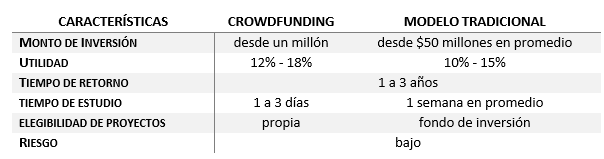
\includegraphics[width=1\linewidth]{imagenes/Tabla} \end{center}

En resumen, las ventajas de la financiación colaborativa, radican inicialmente en la facilidad de acceso, el bajo riesgo, la autonomía inversor para elegir los proyectos, la eliminación de los altos costos de intermediación, mayor utilidad, y el tiempo de estudio de acceso.

\textbf{\emph{GRANJA DE INVERSIONES}}
\textbf{\emph{Autor}}


\includegraphics[width=1\linewidth,height=0.3\textheight]{imagenes/Granja1}

\hypertarget{refs}{}
\begin{cslreferences}
\leavevmode\hypertarget{ref-SAC2019Agricultores}{}%
Agricultores Colombianos, Sociedad de. 2019. ``Colombia: El Mayor Importador Latinoamericano de Productos Agrı́colas Y Alimentos de Estados Unidos.'' \url{https://sac.org.co/colombia-el-mayor-importador-latinoamericano-de-productos-agricolas-y-alimentos-de-estados-unidos/}.

\leavevmode\hypertarget{ref-Portafolio2021Desempleo}{}%
Economı́a, Secciǿn -. 2021. ``Colombia Cerrǿ El 2020 Con Una Tasa de Desempleo En 15,9.'' \emph{Diario Portafolio}. \url{https://www.portafolio.co/economia/tasa-de-desempleo-en-colombia-2020-dane-548662}.

\leavevmode\hypertarget{ref-Ospina2020Colombia}{}%
Ospina Dı́az, N. 2020. ``Crowdfunding' En Colombia: Avanzamos, Pero No Tanto.'' \emph{Mbito Jurı́dico}, 1--6.

\leavevmode\hypertarget{ref-Rojas2021Concejo}{}%
Rojas Mantilla., M. F. 2021. ``El Aumento de La Pobreza En Colombia Es Una Tragedia Social.'' \emph{Concejo de Bogot}. \url{https://concejodebogota.gov.co/el-aumento-de-la-pobreza-en-colombia-es-una-tragedia-social/cbogota/2021-04-30/092932.php}.

\leavevmode\hypertarget{ref-Republica2021millones}{}%
Salazar Sierrra, C. 2021. ``En 2020, 2,78 Millones de Personas Ingresaron a Condiciǿn de Pobreza Extrema.'' \url{https://www.larepublica.co/economia/siga-aqui-la-publicacion-de-las-cifras-del-dane-sobre-la-pobreza-monetaria-en-2020-3161669}.

\leavevmode\hypertarget{ref-Semana2018Apertura}{}%
Semana, Revista. 2018. ``Ası́ Cambiǿ La Economı́a En 28 Años de Apertura.'' \emph{Secciǿn - Comercio Exterior}. \url{https://www.semana.com/economia/articulo/28-anos-apertura-economica/255671/}.
\end{cslreferences}

\end{document}
